\documentclass[zihao=5]{ctexbook}
\setmainfont{SourceSerifPro-Regular}
\usepackage{sourcesanspro}
\usepackage{sourcecodepro}
\setCJKmainfont{SourceHanSerifCN}%
[
	UprightFont = *-Regular,
	BoldFont = *-Bold,
	ItalicFont = 方正新楷体简体,
	BoldItalicFont = *-Bold,
	Mapping = fullwidth-stop
]
\setCJKsansfont{SourceHanSansCN}%
[
	UprightFont = *-Regular,
	BoldFont = *-Bold,
	ItalicFont = *-Regular,
	BoldItalicFont = *-Bold,
	Mapping = fullwidth-stop
]
\setCJKmonofont{SourceHanSansCN}%
[
	UprightFont = *-Regular,
	BoldFont = *-Bold,
	ItalicFont = *-Regular,
	BoldItalicFont = *-Bold,
	Mapping = fullwidth-stop
]
\usepackage{amsmath,amssymb,mwe}
\usepackage[upint]{newtxmath}
\usepackage{upgreek,physics,siunitx}% ,esint
\everymath{\displaystyle}
\edef\iint{\iint\limits}
\usepackage{lastpage}
\usepackage[paperwidth=18cm,paperheight=24cm,left=1cm,right=1cm,top=1.5cm,bottom=1.5cm]{geometry}
\setlength{\headheight}{13pt}

\usepackage{tikz,pgf}
\usetikzlibrary{shapes,calc}
\makeatletter
\newcommand\thumb{%
	\if@mainmatter
	\begingroup
	\catcode`\$=3
	\tikzpicture[remember picture,overlay] % thumb index
	\ifodd\value{page}
	  \node[fill=gray,text=black,anchor=north east,xshift=2mm,
			yshift=-10mm-\arabic{chapter}*20mm,
			shape=semicircle,shape border rotate=90,
			minimum height=10mm,minimum width=5mm,
			font=\normalfont\sffamily\bfseries\Huge]
		at (current page.north east)
		{\llap{\arabic{chapter}\hspace{1mm}}};
	\else
	  \node[fill=gray,text=black,anchor=north west,xshift=-2mm,
			yshift=-10mm-\arabic{chapter}*20mm,
			shape=semicircle,shape border rotate=270,
			minimum height=10mm,minimum width=5mm,
			font=\normalfont\sffamily\bfseries\Huge]
		at (current page.north west)
		{\rlap{\hspace{1mm}\arabic{chapter}}};
	\fi
	\endtikzpicture
	\endgroup
	\fi}
\makeatother

\usepackage{fancyhdr}
\pagestyle{fancy}
\fancyhf{}
\renewcommand{\footrulewidth}{0.4pt}
\fancyhead[RE]{\bfseries \leftmark}
\fancyhead[LO]{\bfseries \rightmark}
\fancyhead[RO,LE]{\thumb}
\fancyhead[C]{\bfseries 仅供学习使用,严禁商业使用}
\fancyfoot[C]{\bfseries --\thepage/\pageref{LastPage}--}
\fancypagestyle{plain}{%
\fancyhf{}
\fancyhead[r]{\thumb}
\fancyfoot[C]{\bfseries --\thepage/\pageref{LastPage}--}
\renewcommand{\headrulewidth}{0pt}
\renewcommand{\footrulewidth}{0pt}}

\usepackage{tcolorbox}
\tcbuselibrary{breakable,skins}
\newtcolorbox[auto counter]{ti}[1][]{%
enhanced,colback=white,colframe=white,attach boxed title to top center={yshift=-0.25mm-\tcboxedtitleheight/2,yshifttext=2mm-\tcboxedtitleheight/2},
boxed title style={
boxrule=0.5mm,frame code={ \path[tcb fill frame] ([xshift=-4mm]frame.west) -- (frame.north west) -- (frame.north east) -- ([xshift=4mm]frame.east) -- (frame.south east) -- (frame.south west) -- cycle; },
interior code={ \path[tcb fill interior] ([xshift=-2mm]interior.west) -- (interior.north west) -- (interior.north east) -- ([xshift=2mm]interior.east) -- (interior.south east) -- (interior.south west) -- cycle;}
},
fonttitle=\bfseries,breakable = false,title=\thetcbcounter,#1}
\usepackage{etoolbox}
% % part A
% \AtEndEnvironment{ti}{\tcblower%
% \parbox[t]{0.5\textwidth}{
% \begin{tabular}[c]{@{}|c|@{}}
% 	\hline
% 	答题\\
% 	区域\\
% 	\hline
% \end{tabular}}%
% \parbox[t]{0.5\textwidth}{%
% \begin{tabular}[c]{@{}|c|@{}}
% 	\hline
% 	纠错\\
% 	笔记\\
% 	\hline
% \end{tabular}
% }
% \\\vspace*{9em}
% }
% % part B
% \AtEndEnvironment{ti}{\tcblower%
% \parbox[t]{\textwidth}{
% \hspace*{\fill}
% \tikz \draw[dashed] (0,0) -- (0,-4);
% \hspace*{\fill}
% }}
\AtBeginEnvironment{tasks}{\kuo{}}
\usepackage{tasks}
\settasks{label=(\Alph*),label-width=15pt,after-item-skip=0pt,debug}
\newcommand{\kuo}{\mbox{(\hspace{1.5em})}}
\newcommand{\hua}{\CJKunderline*[hidden=true]{瞻彼阕者,虚室生白}}
\newcommand{\ee}{\mathrm{e}}
\renewcommand{\leq}{\leqslant}
\renewcommand{\geq}{\geqslant}
\renewcommand{\partial}{\uppartial}
\title{2021 李永乐·王式安考研数学系列\\数学基础过关 660 题 数学一习题册\thanks{Build time:\today}}
\author{李永乐\thanks{清华大学} \and 王式安\thanks{北京理工大学} \and 武忠祥\thanks{西安交通大学}}
\date{2019 年 9 月}
\begin{document}
\frontmatter
\maketitle
\tableofcontents
\mainmatter
\part{基础过关\\1 阶}
\chapter{高等数学}
\section{填空题}
\begin{ti}
	设 $g(x) = \begin{cases}
		2 - x, & x \leq 0 \\
		2 + x, & x > 0
	\end{cases}$, $f(x) = \begin{cases}
		x^{2}, & x < 0 \\
		-x, & x \geq 0
	\end{cases}$,则 $\lim_{x \to 0} g(f(x)) = $ \hua。
\end{ti}

\begin{ti}
	$\lim_{x \to 0}\frac{ \bigl( 1 - \sqrt{\cos x} \bigr) \bigl( 3^{2x} - 1 \bigr) }{\tan(\sin x) \ln (\cos 2x)} = $ \hua。
\end{ti}

\begin{ti}
	$I = \lim_{x \to 0} \frac{ \bigl( \ee^{x^2} - 1 \bigr) \bigl( \sqrt{1 + x} - \sqrt{1 - x} \bigr)  }{ [\ln(1 - x) + \ln(1 + x)] \sin \frac{x}{1+x} } = $ \hua。
\end{ti}

\begin{ti}
	$I = \lim_{x \to +\infty} \biggl( \sin \frac{2}{x} + \cos \frac{1}{x} \biggr)^{x \cos \sqrt{\frac{x+1}{x^{2}}}} = $ \hua。
\end{ti}

\begin{ti}
	$I = \lim_{x \to +\infty} \Bigl( \sqrt[6]{x^{6} + x^{5}} - \sqrt[6]{x^{6} - x^{5}} \Bigr) = $ \hua。
\end{ti}

\begin{ti}
	$I = \lim_{x \to 0} \frac{x \sin x^2 - 2 (1 - \cos x) \sin x}{x^4} = $ \hua。
\end{ti}

\begin{ti}
	$I = \lim_{x \to 0} \frac{\bigl( 1 - \sqrt{\cos x} \bigr) \bigl( 1 - \sqrt[3]{\cos x} \bigr) \cdots \bigl( 1 - \sqrt[n]{\cos x} \bigr)}{(1 - \cos x)^{n-1}} = $ \hua。
\end{ti}

\begin{ti}
	$I = \lim_{x \to \infty} \Bigl( \ee^{x^2} + x^3 \Bigr)^{\frac{1}{x^2}} = $ \hua。
\end{ti}

\begin{ti}
	$I = \lim_{x \to 0} \frac{\int_{x^2}^x \frac{\sin(xt)}{t} \dd{t}}{x^2} = $ \hua。
\end{ti}

\begin{ti}
	设 $a > 0$, $a \ne 1$,且 $I = \lim_{x \to +\infty} x^p \Bigl( a^{\frac{1}{x}} - a^{\frac{1}{x+1}} \Bigr) = \ln a$,则 $p = $ \hua。
\end{ti}

\begin{ti}
	设 $\alpha > 0$,则 $\lim_{x \to 0^{+}} \bigl( x^2 + x \bigr)^{x^\alpha} = $ \hua。
\end{ti}

\begin{ti}
	数列极限 $I = \lim_{n \to \infty} n^2 \biggl( \arctan \frac{2}{n} - \arctan \frac{2}{n+1} \biggr) = $ \hua。
\end{ti}

\begin{ti}
	设 $a$, $b$, $c > 0$,则 $\lim_{x \to 0} \biggl( \frac{a^x + b^x + c^x}{3} \biggr)^{\frac{1}{x}} = $ \hua。
\end{ti}

\begin{ti}
	设 $\lim_{x \to 0} \frac{\ln \Bigl( 1 + x + \frac{f(x)}{x} \Bigr)}{x} = 3$,则 $\lim_{x \to 0} \frac{f(x)}{x^2} = $ \hua。
\end{ti}

\begin{ti}
	设 $\lim_{x \to 0} f(x)$ 存在,并且 $\lim_{x \to 0} \frac{\sqrt{1 + f(x) \sin x} - 1}{\ln(1 + 3x)} = 2$,则 $\lim_{x \to 0} f(x) = $ \hua。
\end{ti}

\begin{ti}
	设函数 $f(x)$ 在 $x = 1$ 连续,且 $f(1) = 1$,则 $\lim_{x \to +\infty} \ln\Bigl[2 + f\Bigl( x^{\frac{1}{x}} \Bigr)\Bigr] = $ \hua。
\end{ti}

\begin{ti}
	设 $a$, $b$ 为常数,且 $\lim_{x \to \infty} \Bigl( \sqrt[3]{1 - x^6} - ax^2 - b \Bigr) = 0$,则 $a = $ \hua,$b = $ \hua。
\end{ti}

\begin{ti}
	设 $a$, $b$, $p$ 为非零常数,则 $I = \lim_{x \to 0} \frac{a + b \ee^{\frac{1}{x}}}{a - b \ee^{\frac{1}{x}}} \cdot \frac{\sin px}{|x|} = $ \hua。
\end{ti}

\begin{ti}
	设 $x_{0} = 0$, $x_{n} = \frac{1 + 2x_{n-1}}{1 + x_{n-1}}$ ($n=1,2,3,\cdots$),则 $\lim_{n \to \infty}x_{n} = $ \hua。
\end{ti}

\begin{ti}
	设 $f(x)$ 连续,$x \to a$ 时 $f(x)$ 是 $x - a$ 的 $n$ 阶无穷小,则 $x \to a$ 时 $\int_a^x f(t) \dd{t}$ 是 $x - a$ 的 \hua{} 阶无穷小。(填阶数)
\end{ti}

\begin{ti}
	已知当 $x \to 0$ 时 $F(x) = \int_0^{x - \sin x} \ln(1+t) \dd{t}$ 是 $x^n$ 的同阶无穷小,则 $n = $ \hua。
\end{ti}

\begin{ti}
	设 $f(x) = \begin{cases}
		\frac{\ln(1 + x^2)}{1 + x^2}, & - \infty < x \leq 1 \\
		A \ee^{\arctan x}, & 1 < x < +\infty
	\end{cases}$, $f(x)$ 在 $(-\infty,+\infty)$ 上连续,则 $A = $ \hua。
\end{ti}

\begin{ti}
	设 $f(x) = \begin{cases}
		6, & x \leq 0 \\
		\frac{\ee^{ax^3} - 1}{x - \arcsin x}, & x > 0
	\end{cases}$, $g(x) = \begin{cases}
		\frac{3 \sin(x - 1)}{x - 1}, & x < 1 \\
		\ee^{bx} + 1, & x \geq 1
	\end{cases}$,若 $f(x) + g(x)$ 在 $(-\infty,+\infty)$ 连续,则 $a = $ \hua{} 且 $b = $ \hua。
\end{ti}

\begin{ti}
	设 $f(x) = \frac{\ee^x - b}{(x-a) (x-b)}$ 有无穷间断点 $x = \ee$,可去间断点 $x = 1$,则 $(a,b) = $ \hua。
\end{ti}

\begin{ti}
	设 $f(x) = \lim_{n \to \infty} \frac{x + x^2 \ee^{nx}}{1 + \ee^{nx}}$,则 $f(x)$ 的连续区间是 \hua。
\end{ti}

\begin{ti}
	设 $f(x) = \begin{cases}
		\arctan x, & x \leq 1 \\
		\frac{1}{2} \bigl( \ee^{x^2 - 1} - x \bigr) + \frac{\uppi}{4}, & x > 1
	\end{cases}$,则 $f'(x) = $ \hua。
\end{ti}

\begin{ti}
	设 $f(x) = \begin{cases}
		\frac{\ln(1 + bx)}{x}, & x \ne 0 \\
		-1, & x = 0
	\end{cases}$,其中 $b$ 为某常数,$f(x)$ 在定义域上处处可导,则 $f'(x) = $ \hua。
\end{ti}

\begin{ti}
	设 $f(x) = \begin{cases}
		x^2, & x \leq 0 \\
		x^\alpha \sin \frac{1}{x}, & x > 0
	\end{cases}$,若 $f(x)$ 可导,则 $\alpha$ 应满足 \hua;若 $f'(x)$ 连续,则 $\alpha$ 应满足 \hua。
\end{ti}

\begin{ti}
	设 $f(x)$ 是以 3 为周期的可导函数且是偶函数,$f'(-2) = -1$,则
	\begin{center}
		$\lim_{h \to 0} \frac{h}{f(5 - 2 \sin h) - f(5)} = $ \hua。
	\end{center}
\end{ti}

\begin{ti}
	设 $f(x)$ 在 $x = 0$ 可导且 $f(0) = 1$, $f'(0) = 3$,则数列极限 $I = \lim_{n \to \infty} \biggl( f\biggl( \frac{1}{n} \biggr) \biggr)^{\frac{\frac{1}{n}}{1 - \cos \frac{1}{n}}} = $ \hua。
\end{ti}

\begin{ti}
	设 $f(x)$ 在 $x = a$ 处二阶导数存在,则
	\begin{center}
		$I = \lim_{h \to 0} \frac{\frac{f(a+h) - f(a)}{h} - f'(a)}{h} = $ \hua。
	\end{center}
\end{ti}

\begin{ti}
	设 $f(x) = x^{\sin x}$ ($x>0$),则 $f'(x) = $ \hua。
\end{ti}

\begin{ti}
	$f(x) = x^2 (x+1)^2 (x+2)^2 \cdots (x+n)^2$,则 $f''(0) = $ \hua。
\end{ti}

\begin{ti}
	设 $y = y(x)$ 由参数方程 $\begin{cases}
		x = \frac{1}{2} \ln \bigl( 1 + t^2 \bigr) \\
		y = \arctan t
	\end{cases}$ 确定,则 $\frac{\dd{y}}{\dd{x}} = $ \hua,$\frac{\dd^2{y}}{\dd{x^2}} = $ \hua。$y = y(x)$ 在任意点处的曲率 $K = $ \hua。
\end{ti}

\begin{ti}
	设 $y = y(x)$ 由方程 $y = \sin(x + y)$ 确定,则 $\frac{\dd^2{y}}{\dd{x^2}} = $ \hua。
\end{ti}

\begin{ti}
	设 $y = x + \ee^x$,则其反函数的二阶导数 $\frac{\dd^2{x}}{\dd{y^2}} = $ \hua。
\end{ti}

\begin{ti}
	设 $f(x) = \int_0^x \ln(1 + \sin t) \dd{t}$,则 $f''(x) = $ \hua。
\end{ti}

\begin{ti}
	设函数 $y = y(x)$ 为由方程 $x^2 + \int_0^y \bigl( 2 + \sin t^2 \bigr) \dd{t} = 1$ 确定的隐函数,则 $\dd{y} = $ \hua。
\end{ti}

\begin{ti}
	设 $y = y(x)$ 在 $(-1,1)$ 二阶可导,满足方程:$\bigl(1 - x^2\bigr) \* \frac{\dd^2{y}}{\dd{x^2}} - x \* \frac{\dd{y}}{\dd{x}} + a^2 \* y = 0$,作变量替换 $x = \sin t$ 后,$y$ 作为 $t$ 的函数满足的方程是 \hua。
\end{ti}

\begin{ti}
	设 $f(x) = \ln \frac{1-2x}{1+3x}$, $n \geq 2$,则 $f^{(n)}(0) = $ \hua。
\end{ti}

\begin{ti}
	设 $y(x) = x^2 \cos 2x$,则 $y^{(10)}(0) = $ \hua。
\end{ti}

\begin{ti}
	设 $y = y(x)$ 是由方程 $2y^3 - 2y^2 + 2xy - x^2 = 1$ 确定的,则 $y = y(x)$ 的极值点是 \hua。
\end{ti}

\begin{ti}
	函数 $y = \frac{(x-3)^2}{4(x-1)}$ 的单调增区间是 \hua,单调减区间是 \hua,极值是 \hua,凹区间是 \hua,凸区间是 \hua。
\end{ti}

\begin{ti}
	设 $(1,3)$ 是曲线 $y = x^3 + ax^2 + bx + 14$ 的拐点,则 $a = $ \hua,$b = $ \hua。
\end{ti}

\begin{ti}
	设 $f(x) = 3x^2 + Ax^{-3}$ ($x > 0$), $A$ 为正常数,则 $A$ 至少为 \hua{} 时,有 $f(x) \geq 20$ ($x > 0$)。
\end{ti}

\begin{ti}
	函数 $f(x) = \bigl| 4x^3 - 18x^2 + 27 \bigr|$ 在 $[0,2]$ 上的最小值等于 \hua,最大值等于 \hua。
\end{ti}

\begin{ti}
	设有界函数 $f(x)$ 在 $(c,+\infty)$ 内可导,且 $\lim_{x \to +\infty} f'(x) = b$,则 $b = $ \hua。
\end{ti}

\begin{ti}
	曲线 $y = \sqrt{4x^2 + x} \ln \biggl( 2 + \frac 1x \biggr)$ 的全部渐近线是 \hua。
\end{ti}

\begin{ti}
	设函数 $f(x)$ 在 $x = 0$ 处连续,且 $\lim_{x \to 0} \frac{f(x)}{\ee^x - 1} = 2$,则曲线 $y = f(x)$ 在 $x = 0$ 处的法线方程为 \hua。
\end{ti}

\begin{ti}
	设 $y = y(x)$ 二阶可导,且 $\frac{\dd{y}}{\dd{x}} = (4 - y) y^\beta$ ($\beta > 0$),若 $y = y(x)$ 的一个拐点是 $(x_0,3)$,则 $\beta = $ \hua。
\end{ti}

\begin{ti}
	设 $\int x^2 f'(x) \dd{x} = \arcsin x + C$,则 $f(x) = $ \hua。
\end{ti}

\begin{ti}
	$I = \int \sqrt{\frac{3-2x}{3+2x}} \dd{x} = $ \hua。
\end{ti}

\begin{ti}
	$I = \int \frac{\sqrt{x+1} + 2}{(x+1)^2 - \sqrt{x+1}} \dd{x} = $ \hua。
\end{ti}

\begin{ti}
	$I = \int \frac{x \ee^x}{\sqrt{1 + \ee^x}} \dd{x} = $ \hua。
\end{ti}

\begin{ti}
	$I = \int \frac{x^4 + 1}{1 + x^6} \dd{x} = $ \hua。
\end{ti}

\begin{ti}
	$I = \int \frac{\sin x}{\sin x + \cos x} \dd{x} = $ \hua。
\end{ti}

\begin{ti}
	$I = \int \frac{\dd{x}}{x \sqrt{x^4 + 1}} = $ \hua。
\end{ti}

\begin{ti}
	设 $f(x) = x^2 - x \int_0^2 f(x) \dd{x} + 2 \int_0^1 f(x) \dd{x}$,则 $f(x) = $ \hua。
\end{ti}

\begin{ti}
	设 $f(x)$ 有一阶导数且满足 $\int_0^1 f(tx) \dd{t} = f(x) + x \sin x$,则 $f(x) = $ \hua。
\end{ti}

\begin{ti}
	$I = \int_0^2 \Biggl( x \sqrt{2x - x^2} - \sqrt{ \biggl( 1 - \frac{1}{4}x^2 \biggr)^3 } \Biggr) \dd{x} = $ \hua。
\end{ti}

\begin{ti}
	设 $f(x)$ 为连续函数,$a$, $b$ 为常数,$a^2 + b^2 \ne 0$, $\int_0^{2\uppi} f(a \cos x + b \sin x) \dd{x} = A \int_{-\frac{\uppi}{2}}^{\frac{\uppi}{2}} f \Bigl( \sqrt{a^2+b^2} \sin x \Bigr) \dd{x}$,则 $A = $ \hua。 
\end{ti}

\begin{ti}
	$f(x) = \begin{cases}
		x \ee^{-x^2}, & x \geq 0 \\
		\frac{1}{1 + \cos x}, & -1 < x < 0
	\end{cases}$,则 $\int_1^4 f(x-2) \dd{x} = $ \hua。
\end{ti}

\begin{ti}
	设 $f(x) = \int_0^{x^2} \ee^{-t^2} \dd{t}$,则 $f(x)$ 的极值为 \hua,$f(x)$ 的拐点坐标为 \hua。
\end{ti}

\begin{ti}
	定积分 $I = \int_0^\uppi \frac{x \sin x}{1 + \cos^2 x} \dd{x} = $ \hua。
\end{ti}

\begin{ti}
	设 $f(x) = \max \bigl\{ 1,x^2 \bigr\}$,则 $\int_1^x f(t) \dd{t} = $ \hua。
\end{ti}

\begin{ti}
	在曲线 $y = x^2$ ($0 \leq x \leq 1$) 上取一点 $\bigl( t,t^2 \bigr)$, ($0 < t < 1$),设 $A_1$ 是曲线 $y = x^2$ ($0 \leq x \leq 1$),直线 $y = t^2$ 和 $x = 0$ 围成的面积;$A_2$ 是由曲线 $y = x^2$ ($0 \leq x \leq 1$) 直线 $y = t^2$ 和 $x = 1$ 围成的面积,则 $t$ 取 \hua{} 时 $A = A_1 + A_2$ 取最小值。
\end{ti}

\begin{ti}
	$\int_1^{+\infty} \frac{\dd{x}}{x \sqrt{2x^2 - 1}} = $ \hua。
\end{ti}

\begin{ti}
	$I = \int_1^{+\infty} \biggl[ \frac{2x^2 + bx + a}{x(2x + a)} - 1 \biggr] \dd{x} = 1$,则 $a = $ \hua,$b = $ \hua。
\end{ti}

\begin{ti}
	$\int_0^{+\infty} \frac{x \ee^{-x}}{(1 + \ee^{-x})^2} \dd{x} = $ \hua。
\end{ti}

\begin{ti}
	摆线 $x = a (t - \sin t)$, $y = a(1 - \cos t)$ ($0 \leq t \leq 2 \uppi$) 与 $x$ 轴围成图形绕 $y = 2a$ 旋转一周而得旋转体的体积 $V = $ \hua。
\end{ti}

\begin{ti}
	设星形线方程为
	\[
		\begin{cases}
			x = a \cos^3 t \\
			y = a \sin^3 t
		\end{cases}
	\]
	则它所围成的面积 $A$ 为 \hua,它的弧长 $L$ 为 \hua,它绕 $x$ 轴旋转而生成的旋转体体积 $V$ 为 \hua,该旋转体的侧面积 $S = $ \hua。
	\begin{center}
		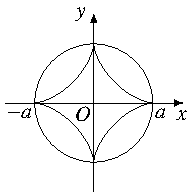
\includegraphics{figure/fig71.pdf}
	\end{center}
\end{ti}

\begin{ti}
	设有曲线 $y = \sqrt{x-1}$,过原点作其切线,则以曲线、切线及 $x$ 轴所围成平面图形绕 $x$ 轴旋转一圈所得到的表面积为 \hua。
\end{ti}

\begin{ti}
	已知抛物叶形线的一部分:
	\[
		y^2 = \frac{x}{9} (3-x)^2 (0 \leq x \leq 3)
	\]
	如图所示,它围成的图形为 $M$,则 $M$ 的面积 $A = $ \hua,$M$ 的质心(形心)$(\bar x,\bar y) = $ \hua。
	\begin{center}
		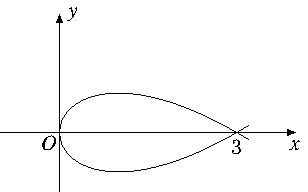
\includegraphics{figure/fig73.pdf}
	\end{center}
\end{ti}

\begin{ti}
	在水平放置的椭圆底柱形容器内储存某种液体,容器的尺寸如图所示,其中椭圆方程为 $\frac{x^2}{4} + y^2 = 1$ (单位:\si{m}),则当液面过点 $(0,y)$ ($-1 \leq y \leq 1$) 处水平线时,容器内液体的体积是 \hua,当容器内储满了液体后,以 \SI{0.16}{m^3/min} 的速度将液体从容器顶端抽出,则当液面降至 $y = 0$ 时,液面下降的速度为 \hua,如果液体的密度为 \SI{1000}{kg/m^3},抽出全部液体所作的功为 \hua。
	\begin{center}
		\includegraphics{example-image}
	\end{center}
\end{ti}

\begin{ti}
	设无穷长直线 $L$ 的线密度为 $1$,引力常数为 $k$,则 $L$ 对距直线为 $a$ 的单位质点 $A$ 的引力为 \hua。
\end{ti}

\begin{ti}
	已知 $y = y(x)$ 在任意点 $x$ 处的增量 $\Delta y = \frac{y \Delta x}{1 + x^2} + \alpha$,其中 $\alpha$ 是 $\Delta x$ 的高阶无穷小($\Delta x \to 0$ 时),$y(0) = \uppi$,则 $y(1) = $ \hua。
\end{ti}

\begin{ti}
	设 $\alpha > 0$ 是常数,连续函数 $f(x)$ 满足 $\lim_{x \to +\infty} f(x) = b$, $y = y(x)$ 是微分方程
	\[
		y' + ay = f(x)
	\]
	的解,则 $\lim_{x \to +\infty} y(x) = $ \hua。
\end{ti}

\begin{ti}
	若通过点 $(1,0)$ 的曲线 $y = y(x)$ 上每一点 $(x,y)$ 处切线的斜率等于 $1 + \frac{y}{x} + \Bigl( \frac{y}{x} \Bigr)^2$,则此曲线的方程是 \hua。
\end{ti}

\begin{ti}
	当 $y > 0$ 时,微分方程 $\bigl( x - 2xy - y^2 \bigr) \dd{y} + y^2 \dd{x} = 0$ 的通解为 \hua。
\end{ti}

\begin{ti}
	微分方程 $yy'' + 2\bigl( y' \bigr)^2 = 0$ 满足初始条件 $y(0) = 1$, $y'(0) = -1$ 的特解是 \hua。
\end{ti}

\begin{ti}
	方程 $y'' + y' - 2y = (6x + 2) \ee^x$ 满足 $y(0) = 3$, $y'(0) = 0$ 的特解 $y^\ast = $ \hua。
\end{ti}

\begin{ti}
	已知连续函数 $f(x)$ 满足 $\int_0^x f(t) \dd{t} = x + \sin x + \int_0^x t f(x-t) \dd{t}$,则 $f(x) = $ \hua。
\end{ti}

\begin{ti}
	设 $y = y(x)$ 是二阶常系数线性微分方程 $y'' + 2my' + n^2y = 0$ 满足 $y(0) = a$ 与 $y'(0) = b$ 的特解,其中 $m > n > 0$,则 $\int_0^{+\infty} y(x) \dd{x} = $ \hua。
\end{ti}

\begin{ti}
	已知 $y_1 = x\ee^x + \ee^{2x}$, $y_2 = x\ee^x + \ee^{-x}$, $y_3 = x\ee^x + \ee^{2x} - \ee^{-x}$ 是某二阶线性非齐次微分方程的三个解,则此微分方程为 \hua。
\end{ti}

\begin{ti}
	设 $u = u \bigl( \sqrt{x^2 + y^2} \bigr)$ ($r = \sqrt{x^2 + y^2} > 0$) 有二阶连续的偏导数,且满足
	\[
		\frac{\partial^2u}{\partial x^2} + \frac{\partial^2u}{\partial y^2} - \frac 1x \frac{\partial u}{\partial x} + u = x^2 + y^2
	\]
	则 $u \bigl( \sqrt{x^2 + y^2} \bigr) = $ \hua。
\end{ti}

\begin{ti}
	设 $f(x,y) = \frac{x^2 + y^2}{\ee^{xy} + xy \sqrt{x^2 + y^2}}$,则 $f_x'(1,0) = $ \hua。
\end{ti}

\begin{ti}
	设 $z = \ee^x + y^2 + f(x+y)$,且当 $y=0$ 时,$z = x^3$,则 $\frac{\partial z}{\partial x} = $ \hua。
\end{ti}

\begin{ti}
	设 $z = (x-2y)^{y-2x}$,则 $\frac{\partial z}{\partial x}\biggl|_{\substack{x=1\\y=0}} = $ \hua。
\end{ti}

\begin{ti}
	设 $f(x,y) = \ln|x + y| - \sin(xy)$,则 $\frac{\partial^2f}{\partial x \partial y}$ 在点 $(1,\uppi)$ 处的值为 \hua。
\end{ti}

\begin{ti}
	设 $f(u,v)$ 是二元可微函数,$z = f\bigl( x^y,y^{2x} \bigr)$,则 $\frac{\partial z}{\partial x} = $ \hua。
\end{ti}

\begin{ti}
	设 $z = \ee^{xy} + f(x+y,xy)$, $f(u,v)$ 有二阶连续偏导数,则 $\frac{\partial^2z}{\partial x \partial y} = $ \hua。
\end{ti}

\begin{ti}
	已知函数 $z = f(x,y)$ 在点 $(1,2)$ 处可微,且 $f(1,2) = 1$, $f_x'(1,2) = 2$, $f_y'(1,2) = 3$,设函数 $\varphi(x) = f(x,2 f(x,2x))$,则 $\varphi'(1) = $ \hua。
\end{ti}

\begin{ti}
	设函数 $f(u,v)$ 具有二阶连续偏导数,且满足 $4 \frac{\partial^2f}{\partial u^2} - \frac{\partial^2f}{\partial v^2} = 1$,又 $g(x,y) = f\bigl(x^2 + y^2,xy \bigr)$,则 $\frac{\partial^2g}{\partial x^2} - \frac{\partial^2g}{\partial y^2} = $ \hua。
\end{ti}

\begin{ti}
	设 $z = \int_0^1 |xy - t| f(t) \dd{t}$, $0 \leq x \leq 1$, $0 \leq y \leq 1$,其中 $f(x)$ 为连续函数,则 $z_{xx}'' + z_{yy}'' = $ \hua。
\end{ti}

\begin{ti}
	设 $f(x)$, $g(x)$ 可微,$u(x,y) = f(2x+5y) + g(2x-5y)$,且满足 $u(x,0) = \sin 2x$, $u_y'(x,0) = 0$,则 $f(x) = $ \hua。
\end{ti}

\begin{ti}
	设 $z = f(x,y)$ 满足 $\frac{\partial^2z}{\partial x \partial y} = x + y$,且 $f(x,0) = x$, $f(0,y) = y^2$,则 $f(x,y) = $ \hua。
\end{ti}

\begin{ti}
	设连续函数 $z = f(x,y)$ 满足 $\lim_{\substack{x \to 0\\y \to 1}} \frac{f(x,y) - 2x + y - 2}{\sqrt{x^2 + (y-1)^2}} = 0$,则 $\dd{z}|_{(0,1)} = $ \hua。
\end{ti}

\begin{ti}
	设 $f(x,y)$ 在点 $(0,0)$ 处连续,且 $\lim_{(x,y) \to (0,0)} \frac{f(x,y) - a - bx - cy}{\ln(1 + x^2 + y^2)} = 1$,其中 $a$, $b$, $c$ 为常数,则 $\dd{f(x,y)}|_{(0,0)} = $ \hua。
\end{ti}

\begin{ti}
	设 $\bigl( ax^2 y^2 - 2xy^2 \bigr) \dd{x} + \bigl( 2x^3 y + bx^2 y + 1 \bigr) \dd{y}$ 是一个函数 $f(x,y)$ 的全微分,则 $a = $ \hua,$b = $ \hua,$f(x,y) = $ \hua。
\end{ti}

\begin{ti}
	设 $f(x,y,z) = \ee^x + y^2 z$,其中 $z = z(x,y)$ 是由方程 $x + y + z + xyz = 0$ 所确定的隐函数,则 $f_x'(0,1,-1) = $ \hua。
\end{ti}

\begin{ti}
	若函数 $z = z(x,y)$ 由方程 $\ee^{x+2y+3z} + xyz = 1$ 确定,则 $\dd{z}|_{(0,0)} = $ \hua。
\end{ti}

\begin{ti}
	设函数 $f(u,v)$ 可微,$z = z(x,y)$ 由方程 $(x+1)z - y^2 = x^2 f(x-z,y)$ 确定,则 $\dd{z}|_{(0,1)} = $ \hua。
\end{ti}

\begin{ti}
	设 $f(x)$ 为连续函数,且 $x^2 + y^2 + z^2 = \int_x^y f(x+y-t) \dd{t}$ 确定二元函数 $z = z(x,y)$,则 $z \biggl( \frac{\partial z}{\partial x} + \frac{\partial z}{\partial y} \biggr) = $ \hua。
\end{ti}

\begin{ti}
	二元函数 $f(x,y) = x^2 \bigl( 2 + y^2 \bigr) + y \ln y$ 的极小值为 \hua。
\end{ti}

\begin{ti}
	设方程式 $x^2 + y^2 + z^2 - 2x - 2y - 4z - 10 = 0$ 确定某隐函数 $z = z(x,y) > 0$,则 $z = z(x,y)$ 的极 \hua{} 值点是 \hua,相应的极值是 \hua。
\end{ti}

\begin{ti}
	设 $a > 0$,交换积分次序 $\int_0^a \dd{y} \int_0^{\sqrt{ay}} f(x,y) \dd{x} + \int_a^{2a} \dd{y} \int_0^{2a-y} f(x,y) \dd{x} = $ \hua。
\end{ti}

\begin{ti}
	交换积分次序 $\int_0^1 \dd{x} \int_0^{x^2} f(x,y) \dd{y} + \int_1^3 \dd{x} \int_0^{\frac{1}{2}(3-x)} f(x,y) \dd{y} = $ \hua。
\end{ti}

\begin{ti}
	将直角坐标中的累次积分转换成极坐标系下的累次积分并计算
	\[
		I = \int_0^{\frac{\sqrt{2}}{2}R} \ee^{-y^2} \dd{y} \int_0^y \ee^{-x^2} \dd{x} + \int_{\frac{\sqrt{2}}{2}R}^R \ee^{-y^2} \dd{y} \int_0^{\sqrt{R^2-y^2}} \ee^{-x^2} \dd{x}
	\]
	$=$ \hua。
\end{ti}

\begin{ti}
	交换积分次序 $\int_{-\frac{\uppi}{4}}^{\frac{\uppi}{2}} \dd{\theta} \int_0^{2 \cos\theta} f(\rho \cos\theta,\rho \sin\theta) \rho \dd{\rho} = $ \hua。
\end{ti}

\begin{ti}
	计算 $\int_0^2 \dd{x} \int_x^2 \ee^{-y^2} \dd{y} = $ \hua。
\end{ti}

\begin{ti}
	计算 $\int_0^1 \dd{x} \int_{x^2}^1 \frac{xy}{\sqrt{1 + y^3}} \dd{y} = $ \hua。
\end{ti}

\begin{ti}
	计算 $\int_0^1 \dd{y} \int_{\arcsin y}^{\uppi - \arcsin y} \cos^2 x \dd{x} = $ \hua。
\end{ti}

\begin{ti}
	计算 $\iint_{x^2+y^2 \leq 1} \bigl( x^2 + 2y \bigr) \dd{\sigma} = $ \hua。
\end{ti}

\begin{ti}
	计算 $\int_0^a \dd{x} \int_0^{\sqrt{a^2-x^2}} \sqrt{x^2 + y^2} \dd{y} = $ \hua。
\end{ti}

\begin{ti}
	设 $D = \{ (x,y) | 0 \leq x \leq 1,0 \leq y \leq 1 \}$,则 $\iint_{D} \frac{\dd{x}\dd{y}}{\sqrt{x^2+y^2}} = $ \hua。
\end{ti}

\begin{ti}
	设 $D = \{ (x,y) | -1 \leq x \leq 1,0 \leq y \leq 2 \}$,则 $I = \iint_{D} \sqrt{|y - x^2|} \dd{x}\dd{y} = $ \hua。
\end{ti}

\begin{ti}
	设 $f(x)$ 为连续函数,$F(x) = \int_1^x \dd{v} \int_v^x f(u) \dd{u}$ ($x > 1$),则 $F'(x) = $ \hua。
\end{ti}

\begin{ti}
	设 $f(x,y)$ 为连续函数,且 $f(x,y) = \frac{1}{\uppi} \sqrt{x^2 + y^2} \iint_{x^2+y^2 \leq 1} f(x,y) \dd{\sigma} + y^2$,则 $f(x,y) = $ \hua。
\end{ti}

\begin{ti}
	设积分区域 $D = \bigl\{ (x,y) \bigl| 1 \leq x^2+y^2 \leq \ee^2 \bigr\}$,则 $\iint_{D} x^2 \ln \bigl(x^2+y^2\bigr) \dd{\sigma} = $ \hua。
\end{ti}

\begin{ti}
	设积分区域 $D$ 由曲线 $y = \ln x$ 以及直线 $x = 2$, $y = 0$ 围成,则 $\iint_{D} \frac{\ee^{xy}}{x^x - 1} \dd{\sigma} = $ \hua。
\end{ti}
\section{选择题}
\begin{ti}
	设有下列命题
	\begin{tasks}[label=(\arabic*)]
		\task 数列 $\{ x_n \}$ 收敛(即 $\exists$ 极限 $\lim_{n \to \infty} x_n$),则 $x_n$ 有界。
		\task 数列极限 $\lim_{n \to \infty} x_n = a \Leftrightarrow \lim_{n \to \infty} x_{n+l} = a$。其中 $l$ 为某个确定的正整数。
		\task 数列 $\lim_{n \to \infty} x_n = a \Leftrightarrow \lim_{n \to \infty} x_{2n-1} = \lim_{n \to \infty} x_{2n} = a$。
		\task 数列极限 $\lim_{n \to \infty} x_n \exists \Leftrightarrow \lim_{n \to \infty} \frac{x_{n+1}}{x_n} = 1$。
	\end{tasks}
	则以上命题中正确的个数是
	\begin{tasks}(4)
		\task 1。
		\task 2。
		\task 3。
		\task 4。
	\end{tasks}
\end{ti}

\begin{ti}
	设 $x_n \leq z_n \leq y_n$,且 $\lim_{n \to \infty} (y_n - x_n) = 0$,则 $\lim_{n \to \infty} z_n$
	\begin{tasks}(2)
		\task 存在且等于零。
		\task 存在但不一定等于零。
		\task 不一定存在。
		\task 一定不存在。
	\end{tasks}
\end{ti}

\begin{ti}
	有以下命题:设 $\lim_{x \to a} f(x) = A$, $\lim_{x \to a} g(x)$ 不 $\exists$, $\lim_{x \to a} h(x)$ 不 $\exists$,
	\begin{tasks}[label=(\arabic*)](2)
		\task $\lim_{x \to a} (f(x) \cdot g(x))$ 不 $\exists$。
		\task $\lim_{x \to a} (g(x) + h(x))$ 不 $\exists$。
		\task $\lim_{x \to a} (h(x) \cdot g(x))$ 不 $\exists$。
		\task $\lim_{x \to a} (g(x) + f(x))$ 不 $\exists$。
	\end{tasks}
	则以上命题中正确的个数是
	\begin{tasks}(4)
		\task 0。
		\task 1。
		\task 2。
		\task 3。
	\end{tasks}
\end{ti}

\begin{ti}
	下列叙述正确的是
	\begin{tasks}
		\task 如果 $f(x)$ 在 $x_0$ 的任意空心邻域内无界,则 $\lim_{x \to x_0} f(x) = \infty$。
		\task 如果 $\lim_{x \to x_0} f(x) = \infty$,则 $f(x)$ 在 $x_0$ 的任意空心邻域内无界。
		\task $\lim_{x \to x_0} f(x)$ 不存在,则 $\lim_{x \to x_0} f(x) = \infty$。
		\task 如果 $\lim_{x \to x_0} f(x) = 0$,则 $\lim_{x \to x_0} \frac{1}{f(x)} = \infty$。
	\end{tasks}
\end{ti}

\begin{ti}
	下列命题中正确的是
	\begin{tasks}
		\task 若 $\lim_{x \to x_0} f(x) \geq \lim_{x \to x_0} g(x) \Rightarrow \exists \delta > 0$,当 $0 < |x-x_0| < \delta$ 时 $f(x) \geq g(x)$。\xeCJKnobreak
		\task 若 $\exists \delta > 0$ 使得当 $0 < |x-x_0| < \delta$ 时有 $f(x) > g(x)$ 且 $\lim_{x \to x_0} f(x) = A_0$, $\lim_{x \to x_0} g(x) = B_0$ 均 $\exists$,则 $A_0 > B_0$。
		\task 若 $\exists \delta > 0$,当 $0 < |x-x_0| < \delta$ 时 $f(x) > g(x) \Rightarrow \lim_{x \to x_0} f(x) \geq \lim_{x \to x_0} g(x)$。\xeCJKnobreak
		\task 若 $\lim_{x \to x_0} f(x) \geq \lim_{x \to x_0} g(x) \Rightarrow \exists \delta > 0$,当 $0 < |x-x_0| < \delta$ 时有 $f(x) > g(x)$。
	\end{tasks}
\end{ti}

\begin{ti}
	$\lim_{n \to \infty} \sin^2\bigl( \uppi \sqrt{n^2+n} \bigr) = $
	\begin{tasks}(4)
		\task $1$。
		\task $\frac{3}{4}$。
		\task $\frac{1}{2}$。
		\task $\frac{1}{4}$。
	\end{tasks}
\end{ti}

\begin{ti}
	当 $n \to \infty$ 时,$\ee - \biggl(1 + \frac{1}{n}\biggr)^n$ 与 $An^{-p}$ 为等价无穷小,则
	\begin{tasks}(2)
		\task $A = \frac{\ee}{3}$, $p = 1$。
		\task $A = \frac{\ee}{2}$, $p = 1$。
		\task $A = \frac{\ee}{3}$, $p = 2$。
		\task $A = \frac{\ee}{2}$, $p = 2$。
	\end{tasks}
\end{ti}

\begin{ti}
	$\lim_{n \to \infty} \biggl( \frac{1}{n^2+n+1} + \frac{2}{n^2+n+2} + \cdots + \frac{n}{n^2+n+n} \biggr) = $
	\begin{tasks}(4)
		\task $3$。
		\task $2$。
		\task $\frac{2}{3}$。
		\task $\frac{1}{2}$。
	\end{tasks}
\end{ti}

\begin{ti}
	$f(x) = \frac{\sin \uppi x}{x-1} \ee^{\frac{1}{(x-1)^3}}$,则当 $x \to 1$ 时有
	\begin{tasks}
		\task $\lim_{x \to 1} f(x) = - \uppi$。
		\task $\lim_{x \to 1} f(x) = 0$。
		\task $\lim_{x \to 1} f(x) = \infty$。
		\task $\lim_{x \to 1} f(x)$ 不存在,且 $\lim_{x \to 1} f(x) \ne \infty$。
	\end{tasks}
\end{ti}

\begin{ti}
	$I = \lim_{x \to 0} \frac{\cos( x\ee^x ) - \ee^{-\frac{x^2}{2} \ee^{2x}}}{x^4} = $
	\begin{tasks}(4)
		\task $0$。
		\task $-\frac{1}{6}$。
		\task $-\frac{1}{8}$。
		\task $-\frac{1}{12}$。
	\end{tasks}
\end{ti}

\begin{ti}
	$\lim_{x \to \infty} \biggl( \cos\frac{1}{x} \biggr)^{x^2} = $
	\begin{tasks}(4)
		\task 1。
		\task $\ee$。
		\task $\ee^{\frac{1}{2}}$。
		\task $\ee^{-\frac{1}{2}}$。
	\end{tasks}
\end{ti}

\begin{ti}
	$\lim_{x \to 0} \frac{\cos(\sin x) - \cos x}{(1 - \cos x) \sin^2x} = $
	\begin{tasks}(4)
		\task $1$。
		\task $\frac{1}{2}$。
		\task $\frac{1}{3}$。
		\task $0$。
	\end{tasks}
\end{ti}

\begin{ti}
	$\lim_{x \to +\infty} \frac{\bigl( 1 + \frac{1}{x} \bigr)^{x^2}}{\ee^x} = $
	\begin{tasks}(4)
		\task $0$。
		\task $\ee^{-\frac{1}{4}}$。
		\task $\ee^{-\frac{1}{3}}$。
		\task $\ee^{-\frac{1}{2}}$。
	\end{tasks}
\end{ti}

\begin{ti}
	已知 $I = \lim_{x \to 0} \frac{ax^2 + bx + 1 - \ee^{x^2-2x}}{x^2} = 2$,则
	\begin{tasks}(2)
		\task $a = 5$, $b = -2$。
		\task $a = -2$, $b = 5$。
		\task $a = 2$, $b = 0$。
		\task $a = 3$, $b = -3$。
	\end{tasks}
\end{ti}

\begin{ti}
	设 $\lim_{x \to 0} \frac{\sin 6x - (\sin x) f(x)}{x^3} = 0$,则 $\lim_{x \to 0} \frac{6-f(x)}{x^2} = $
	\begin{tasks}(4)
		\task $0$。
		\task $35$。
		\task $36$。
		\task $\infty$。
	\end{tasks}
\end{ti}
\end{document}